\documentclass{article}

% if you need to pass options to natbib, use, e.g.:
% \PassOptionsToPackage{numbers, compress}{natbib}
% before loading nips_2017
%
% to avoid loading the natbib package, add option nonatbib:
% \usepackage[nonatbib]{nips_2017}

%\usepackage{main}

% to compile a camera-ready version, add the [final] option, e.g.:
\usepackage[final]{main}

\usepackage[utf8]{inputenc} % allow utf-8 input
\usepackage[T1]{fontenc}    % use 8-bit T1 fonts
\usepackage{hyperref}       % hyperlinks
\usepackage{url}            % simple URL typesetting
\usepackage{booktabs}       % professional-quality tables
\usepackage{amsfonts}       % blackboard math symbols
\usepackage{nicefrac}       % compact symbols for 1/2, etc.
\usepackage{microtype}      % microtypography
\usepackage{multicol}
\usepackage{graphicx}
\usepackage{amsmath}
\usepackage{bbm}
\usepackage{enumerate}
\usepackage[linguistics]{forest}
\usepackage{adjustbox}
\usepackage{bbm}
\usepackage{stmaryrd}
%\usepackage[margin=0.5in]{geometry}
%\DeclareMathOperator*{\argmax}{argmax}

\usepackage{listings}
\lstset{
  basicstyle=\ttfamily,
  mathescape
}
\usepackage{color}
 
\definecolor{codegreen}{rgb}{0,0.6,0}
\definecolor{codegray}{rgb}{0.5,0.5,0.5}
\definecolor{codepurple}{rgb}{0.58,0,0.82}
\definecolor{backcolour}{rgb}{0.95,0.95,0.92}
 
\lstdefinestyle{mystyle}{
    backgroundcolor=\color{backcolour},   
    commentstyle=\color{codegreen},
    keywordstyle=\color{magenta},
    numberstyle=\ttfamily\tiny\color{codegray},
    stringstyle=\color{codepurple},
    basicstyle=\ttfamily\small,
    columns=fullflexible,
    breakatwhitespace=false,         
    breaklines=true,                 
    captionpos=t,                    
    keepspaces=true,                 
    numbers=left,                    
    numbersep=5pt,                  
    showspaces=false,                
    showstringspaces=false,
    showtabs=false,                  
    tabsize=4,
}
 
\lstset{style=mystyle}

\title{Fundamental Algorithms - Spring 2018\\
       \Large Homework 8}
\graphicspath{{images/}}
\setcitestyle{round, sort, numbers}

% The \author macro works with any number of authors. There are two
% commands used to separate the names and addresses of multiple
% authors: \And and \AND.
%
% Using \And between authors leaves it to LaTeX to determine where to
% break the lines. Using \AND forces a line break at that point. So,
% if LaTeX puts 3 of 4 authors names on the first line, and the last
% on the second line, try using \AND instead of \And before the third
% author name.

\author{
  Daniel Rivera Ruiz\\
  Department of Computer Science\\
  New York University\\
  \href{mailto:drr342@nyu.edu}{\texttt{drr342@nyu.edu}}\\
}

\begin{document}

\maketitle

% \cite{} - in-line citation author, year in parenthesis.
% \citep{} - all citation info in parenthesis.

%	\begin{figure}[ht]
%		\centering
%		\frame{
%            \includegraphics[width=1.0\linewidth]{tree.png}
%       }
%		\caption{Classification results for the sentence \textit{"There are slow and repetitive parts, but it has just enough spice to keep it                  interesting."} using the Stanford Sentiment Treebank. As can be seen, sentiment scores are available for each phrase.}
%		\label{tree}
%	\end{figure}

\begin{enumerate}[1.]

    \item The following is the pseudocode for the algorithm:
\begin{lstlisting}
    R[0] = 0
    for j = 1 to $N^2$:
        R[j] = 0
        for k = 1 to W:
            TEMP = PRICE[k] + R[j - k]
            if (R[j] < TEMP):
                R[j] = TEMP
            end if
        end for
    end for
    return R[$N^2$]
\end{lstlisting}

    All the operations executed in the inner \texttt{for} loop of the algorithm take constant time, so its time complexity is $O(W)$. The outer \texttt{for} loop is executed $N^2$ times, so the overall time complexity of the algorithm is:
    \begin{align*}
        T(N) &= N^2 \cdot O(W)\\
        T(N) &= O(N^2W)\\
        T(N) &= O(N^2 \left \lfloor{\sqrt{N}}\right \rfloor)\\
        T(N) &= O(N^{\frac{5}{2}})
    \end{align*}
    
    The algorithm works as follows:
    \begin{itemize}
        \item On line 1 we establish the base case $R[0] = 0$.
        \item On lines 2 through 10, we iterate over all the possible values of $j$ to get the revenue values $R$.
        \item Line 3 initializes $R[j]$ to zero (assuming that it is the minimum value the revenue can take).
        \item Lines 4 through 9 define the position of the first cut in the rod based in the conditions of the problem: 1) the rod lengths must be at most $W$ (hence the \texttt{for} loop from 1 to $W$) and 2) we want to maximize the total revenue. So while we traverse the loop, we compute the revenue produced by making the first cut at position $k$ which is equals to $P[k] + R[j - k]$. If this value is bigger than the current value of $R[j]$ we update it.
        \item Finally, on line 11 we return the desired value $R[N^2]$.
    \end{itemize}
    
    \item Lets suppose that the frequency for $z$ is less than $\frac{1}{3}$ and $z$ has an encoding of length 1. This means that $z$ must not merge with any other node until the end of the Huffman algorithm. If we look at the last stage where there are only tree elements left, the other two elements (lets call them $a$ and $b$) must merge to form another node so that $z$ still corresponds to a codeword of length 1. At this point we have $f(z) + f(a) + f(b) = 1$ and $f(z) < \frac{1}{3}$, which implies $f(a) + f(b) > \frac{2}{3}$.\\
    The last inequality entails that at least one of $f(a)$ or $f(b)$ must be greater than $\frac{1}{3}$, but in that case according to the Huffman algorithm they wouldn't merge, since choosing $z$ and $argmin(f(a), f(b))$ would yield a better solution. This leads to a contradiction of the original assumption, which means that for any character to be encoded in length one, it must have frequency at least $\frac{1}{3}$.\\
    The following tree is an example for $f(z) = 0.36$ with $z$ encoded as $0$:
    
	\begin{center}
      \begin{forest}
        [\text{$1$}
            [\textit{$z:0.36$}]
            [\text{$0.64$}
                [\text{$0.22$}
                    [\textit{$v:0.10$}]
                    [\textit{$w:0.12$}]]
                [\text{$0.42$}
                    [\textit{$x:0.20$}]
                    [\textit{$y:0.22$}]]]]
      \end{forest}
    \end{center}
    
    \item Selecting the last activity to start that is compatible with all previously selected activities will traverse the time available for the activities in a "backward" manner, appending to the optimal set the activity that leaves more time available for other activities at the beginning of the time interval. This algorithm is optimal because the intuition behind it is the same as for the original one, in the sense that they both try to maximize the time interval left after selecting an activity (the original algorithm selects the activity that ends first, leaving more time at the end of the interval).\\
    The following is the pseudocode for the modified algorithm, where $s$ is an array containing the starting times of the activities (in monotonically decreasing order) and $f$ is the corresponding array with the finishing times:
    
\begin{lstlisting}
Greedy-Activity-Selector-2(s, f):
    n = s.length
    A = {$a_1$}
    k = 1
    for m = 2 to n:
        if f[m] $\leq$ s[k]:
            A = A $\cup$ {$a_m$}
            k = m
        end if
    end for
    return A
\end{lstlisting}

    \item 
    \begin{enumerate}[(a)]
        \item The following figure shows a counterexample for a small problem with four activities: selecting the shortest activity first would yield $a_1$, which only leaves room for $a_4$. This is clearly not optimal, since the set $A = \{a_2, a_3, a_4\}$ is also feasible and has more activities.
    	\begin{figure}[ht]
    		\centering
    		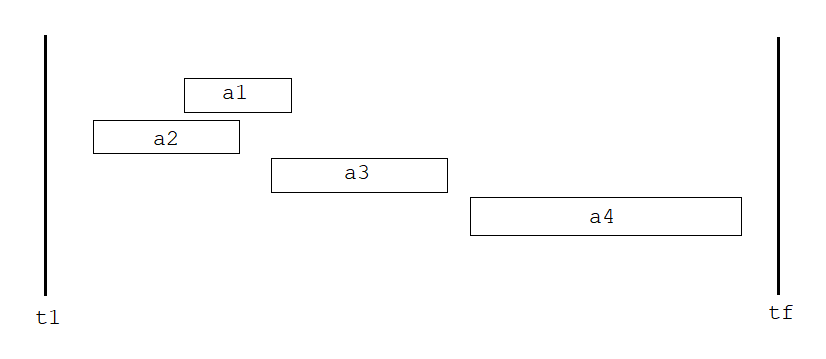
\includegraphics[width=1.0\linewidth]{Shortest.PNG}
    		\caption{Counterexample for shortest activity selection.}
    		\label{diagrams}
    	\end{figure}
        \item
        \item Counterexample: the activity $a_i$ with the earliest starting time has the longest duration of all the remaining activities. In such a case, selecting $a_i$ would not yield an optimal solution because a lot of time would be allocated to only that activity. Since the optimization problem is concerned with the amount of activities selected, it would be better to select more activities with shorter duration times.
    \end{enumerate}
    
    \item
    \begin{enumerate}[(a)]
        \item The following table shows an optimal Huffman code for the eight characters associated to the first eight Fibonacci numbers:
    	\begin{table}[ht]
    		\centering
    		\begin{tabular}{cccl}
    			\toprule
    			$i$ & $a_i$ & $F_i$ & Encoding \\
    			\midrule
                1 & a & 1 & 1111111 \\
                2 & b & 1 & 1111110 \\
                3 & c & 2 & 111110 \\
                4 & d & 3 & 11110 \\
                5 & e & 5 & 1110 \\
                6 & f & 8 & 110 \\
                7 & g & 13 & 10 \\
                8 & h & 21 & 0 \\
    			\bottomrule
    		\end{tabular}
	    \end{table}
    	
    	\item The generalization of the previous exercise to $n$ letters with frequencies equal to the first $n$ Fibonacci numbers is as follows: \emph{the first element is encoded as $(n-i)$ ones, and for all other values of $i$, the $i^{th}$ element is encoded as $(n-i)$ ones plus a trailing zero.}\\
    	The following table and tree show this generalization:
    	\begin{table}[ht]
    		\centering
    		\begin{tabular}{cccl}
    			\toprule
    			$i$ & $a_i$ & $F_i$ & Encoding \\
    			\midrule
                1 & $a_1$ & 1 & $\overbrace{1 \ldots 1}^\text{n - 1}$ \\
                2 & $a_2$ & 1 & $\overbrace{1 \ldots 1}^\text{n - 2}0$ \\
                3 & $a_3$ & 2 & $\overbrace{1 \ldots 1}^\text{n - 3}0$ \\
                $\ldots$ & $\ldots$ & $\ldots$ & $\ldots$ \\
                $n-1$ & $a_{n-1}$ & $F_{n-1}$ & 10 \\
                $n$ & $a_n$ & $F_n$ & 0 \\
    			\bottomrule
    		\end{tabular}
	    \end{table}

	\begin{center}
      \begin{forest}
        [\text{$(F_{n + 2}) - 1$}
            [\text{$a_n:F_n$}]
            [\text{$(F_{n + 1}) - 1$}
                [\text{$a_{n-1}:F_{n-1}$}]
                [\ldots
                    [\text{$a_3:F_3 = 2$}]
                    [\text{$(F_4) - 1 = 2$}
                        [\text{$a_2:F_2 = 1$}]
                        [\text{$a_1:F_1 = 1$}]]]]]
      \end{forest}
    \end{center}
    \end{enumerate}
    
    \item If we used the "standard" method to implement the Huffman code, instead of using a Min-Heap we would have to keep a sorted array with the frequencies of the characters. The time complexity analysis would be as follows:
    \begin{enumerate}[(a)]
        \item The original sorting of the frequencies would take $O(n \log n)$ time.
        \item The two \texttt{Extract-Min} steps would take constant time $O(1)$.
        \item The \texttt{Insert} step would take linear time $O(n - i)$, since we would have to traverse the array to find the correct position for the new frequency.
    \end{enumerate}
    Steps $(b)$ and $(c)$ are executed inside a for loop with values of $i$ from 1 to $n-1$, and therefore the overall time complexity becomes:
    \begin{align*}
        T(n) &= O(n \log n) + O\left(\sum_{i = 1}^{n-1}\left(1 + n - i\right)\right)\\
        T(n) &= O(n \log n) + O\left((n-1) + (n-1)(n) - \frac{(n-1)(n)}{2}\right) \\
        T(n) &= O(n^2)
    \end{align*}
    
\end{enumerate}
\end{document}